\documentclass[]{usiinfbachelorproject}

\captionsetup{labelfont={bf}}

\author{Francesco Costa}

\title{Implementing Fluid Dynamic Simulation using DPD Method}
\subtitle{}
\versiondate{\today}

\begin{committee}
%With more than 1 advisor an error is raised...: only 1 advisor is allowed!
\advisor[Universit\`a della Svizzera Italiana, Switzerland]{Prof.}{Antonio}{Carzaniga}
%You can comment out  these lines if you don't have any assistant
% \assistant[Universit\`a della Svizzera Italiana, Switzerland]{Title}{AssistantName1}{AssistanSurname1}
% \assistant[Universit\`a della Svizzera Italiana, Switzerland]{Title}{AssistantName2}{AssistanSurname2}
\end{committee}

\abstract {
Digital simulations are useful tools to visualize results, extract information and simulate physical phenomena.
There are many methods that can be used to create simulations and each have their own advantages and flaws. One main 
characteristic to differentiate these types is the length-scale: atomistic models can be used to represent 
materials and physical objects at the atomic level, leading to precise but computationally expensive simulations;
macroscopic models are focused instead on bigger systems, with the advantage of being less computationally demanding. DPD 
(Dissipative Particle Dynamics) is a method that stands in between the aforementioned scales. By considering groups of atoms as 
particles we can simulate a fluid in a real time simulation (which would usually be done only in static environments with fixed objects).
The aim of this project is to extend an existing physics simulation tool by implementing the DPD method.
Simulations of this type are used in a number of different fields, such as the medical one (simulating blood flow in vessels).
In our case the purpose of this tool is to mainly be used for didactic means, to show the power and possibilities of informatics.
}

\begin{document}
\maketitle

\tableofcontents

\newpage

%%%%%%%%%%%%%%%%%%%%%%%%%
\section{Introduction} \label{introduction}
%%%%%%%%%%%%%%%%%%%%%%%%%

Simulating consists in the process of imitating a system or real-world
phenomena. This can be done in many different ways but requires in general 
one or multiple models that represent the behaviour of the target in the 
simulation. The choice of such model and its definition are key to create 
an environment which provides valid and reliable results.

There are a number of fields that make extensive use of simulations for 
different reasons. In some cases, such as for engineering, the system of 
interest may be dangerous to test, or it may still not have been built. 
Using simulations allows to test a system before it goes in production, 
decreasing time and cost in the development stage by applying the trial 
and error method in a controlled and flexible environment. There is in general 
an interest in modeling natural systems (a physic system in the case of this project), as well as 
human systems (commonly economics). This need brought forward an increasing necessity of 
bigger and more complex simulations, leading us to the role of informatics and computer simulations.

\subsection{Computer Simulations}
The power of informatics in the context of simulating is the prime example of 
why it is important for workers and researchers in different fields to learn 
the basics of computer science and programming. Depending on the complexity and 
suitability of the model it is possible to simulate virtually any system (accepting 
in some cases higher degrees of approximation). Another advantage of digital simulations 
is the possibility of visualizing the results using computer graphics techniques.

Most simulations of natural systems are based on physical laws, thus reducing the problem 
to the definition of a physics engine. While in general simple physical laws can be reproduced 
in software, there are cases in which it is only possible (or advised) to use approximations and 
simplifications in order obtain better performance. The cost of the simulation and the computational 
power available act as a limit in the way certain phenomena can be modeled. Real-time simulations 
are based on models that can execute at the same time as the real-world system, allowing to observe very 
realistic simulations. The problem with this approach is the computational strain that is forced onto 
the machine running the program, which means that for certain complex simulations either a really powerful 
machine or a very efficient model and code are required.

\subsection{Approaches} \label{Approaches}
Simulations can vary in kind vastly depending on the system they are based on. One big distinction 
can be made when talking about imitating natural systems and that is length-scale. A simulation of a 
chemical compund to the atomic level will be very different from one representing the effect of gravity 
on rigid bodies. This difference can be categorized in three main classes:

\begin{description}
    \item[Atomistic scale] Simulations of this length-scale aim to study the 
    composition of matter itself, resulting in usually computationally expensive processes.
    The main fields implementing such models are biology, chemistry and physics, especially when the 
    three disciplines intertwine.
    \item[Macroscopic scale] When describing the global state of a system we don't focus 
    on the single elements but rather on generalizing the dynamics of the phenomena. The model 
    usually consists of sets of equation describing the system (such as equations of motion for Mechanics and Kinematics).
    \item[Middleground between scales] There are cases in which we would want to describe matter in fine 
    detail without incurring in excessive execution cost. One solution to this problem is to consider particles instead of atoms.
    These particles are agglomerates of atoms which allow for reasonably precise control of interaction between 
    the elements of the system as well as a good overall representation of the global state. Using a method built 
    on such a length-scale allows for example to simulate hydrodynamic behaviour at a much lower cost.
\end{description}

Fluid Dynamics being a focal point of this project it is important to talk about 
the difference between CFD (computational fluid dynamics) simulations and real-time 
simulations. In CFD the objective is to imitate the behaviour of a fluid usually around static 
objects. This is done to study the characteristics of both elements in the simulation.
If we want to consider instead the fluid as an environmental effect, we would want to be 
able to simulate foreign bodies moving in such fluid. This is not possible with the standard CFD 
approach since the cost of emulating the fluid is too high to be incorporated in a real-time simulation.
The method used for this project allows for such a simulation without compromising excessively on the 
behaviour of the fluid.

\newpage
\subsection{Goal of the project}
The goal of this project was to extend an existing tool consisting of a simple physics engine 
capable of modeling the effect of gravity on 2D spheres and the collision between those bodies.
The choice of direction for the extension was influenced by my interest in the topic 
of fluid dynamics and by being introduced to the method used by Professor Pivkin. 
The purpose of the tool also played a major role in the design process, since 
as a didactic tool to showcase the possibilities of computer programs it was most important 
to aim for a visually interesting and pleasing result. This fact didn't diminish nontheless the 
interest in also applying and validating the particular method used for modeling.

\newpage
\section{Fluid Dynamics Simulations}
Fluid mechanics is a branch of physics concerned with the behaviour of fluids (such as liquids or gases) 
when forces are applied to them. Given our objective and the nature of simulations we will mainly 
focus on the dynamics of fluids. The study of the motion of a fluid involves the correlation of many of its 
properties such as velocity, density, pressure and temperature. The results of such models are used 
in a number of different disciplines like (most commonly) aerodynamics and hydrodynamics.

\subsection{CFD Simulations}
The most common way to model a fluid is through Computational Fluid Dynamics (or CFD) simulations, which, as introduced in 
\ref{Approaches}, allow to reproduce the bahaviour of a fluid in an extremely detailed way. The cost of modeling systems using this 
method is usually expensive, hence making CFD not suitable for real-time applications such as the one developed in this project.
The theory and application of this method still makes it worthwhile to study since it gives better insight 
on why other approaches may or may not work and why they may work better in certain scenarios.

\begin{figure} [h]
    \centering
    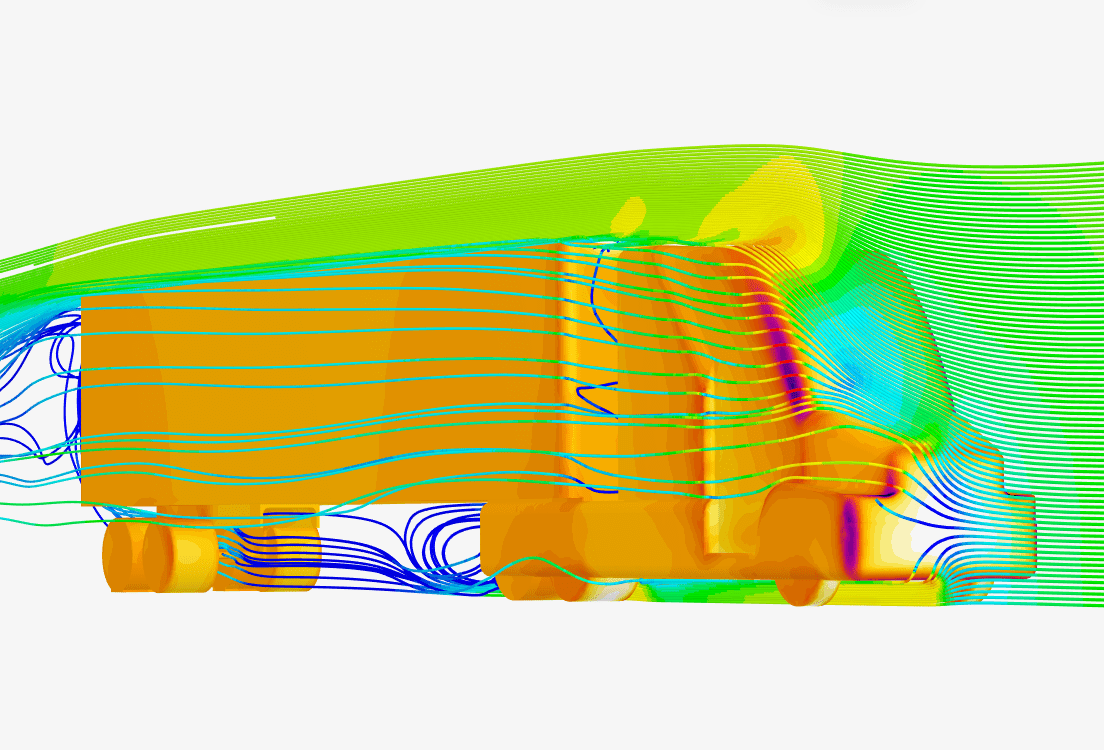
\includegraphics[width=0.5\textwidth]{CFD.png}
    \caption{CFD simulation of fluid (Taken from SimScale)}
    \label{fig:CFDsim}
\end{figure}

As the name would suggest CFD is a technique based on mathematical computation and numerical analysis, which explains why 
powerful computers are necessary to create and handle the simulations. The complexity of the system to be modeled is directly 
correlated to the computing power required to simulate it.

In the following section a theoretical backgorund on the implementation of this method is given in 
order to accustom the reader to the crucial recurring elements of fluid dynamics.

\subsubsection{Navier-Stokes Equations}
The Navier-Stokes equations are differential equations used to describe the behaviour of a fluid at a specific 
point and time. The solution of the equations is effectively a vector field for the velocity of the fluid in each point of interest.
\begin{figure} [h]
    \centering
    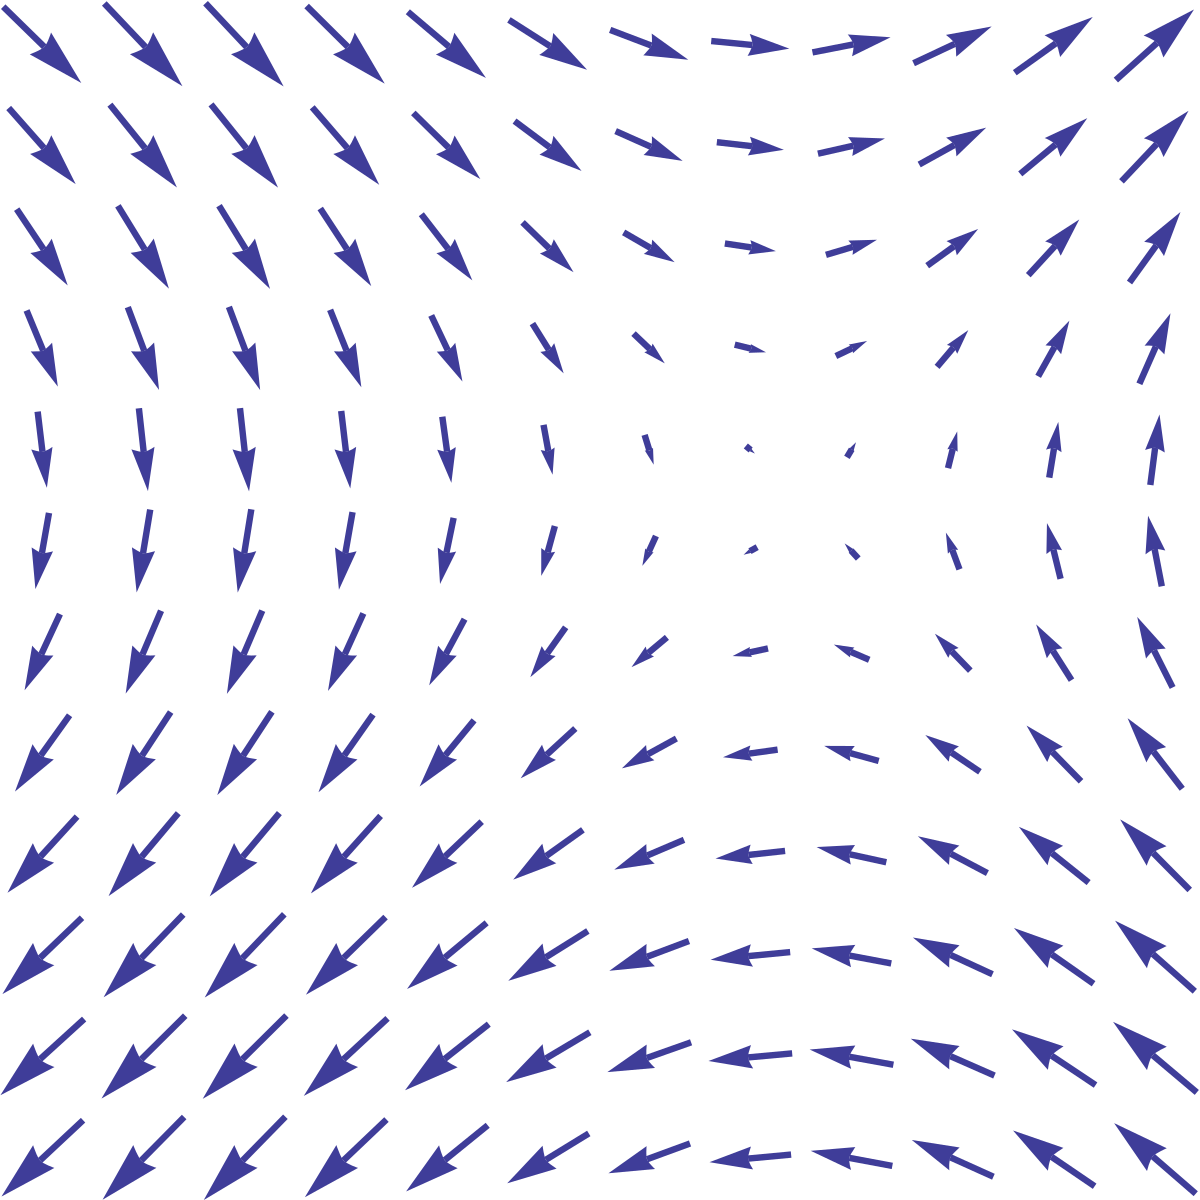
\includegraphics[width=0.3\textwidth]{VectorField.png}
    \caption{Vector Field to represent for example velocity in each point (Taken from Wikipedia)}
    \label{fig:VectorField}
\end{figure}
Given the velocity field the equations can also relate the other important elements characterizing fluids, namely pressure, 
temperature and density. The Navier-Stokes equations for an incompressible fluid with velocity field $\vec{u}$ are 

$$ \frac{\partial \vec{u}}{\partial t} + (\vec{u} \cdot \nabla) \vec{u} = - \frac{1}{\rho} \nabla p + v \nabla^2 \vec{u}$$

where 
\begin{itemize}
    \item $t$ is the time;
    \item $\nabla$ is the divergence (which operates on a vector field to give a scalar field);
    \item $\rho$ is the density;
    \item $p$ is the pressure;
    \item $v$ is the kinematic viscosity (which correlates the dynamic viscosity to the density of the fluid).
\end{itemize}

Depending on which fluid we are trying to model the Navier-Stokes equations change following the properties of the fluid, but for most cases 
they remain eqautions for which the solution can only be found with the help of computers.

\subsection{DPD Method}
Dissipative particle dynamics (or DPD) is a simulation method first introduced by Hoogerbrugge and Koelman \cite{Hoogerbrugge} used to 
model hydrodynamic behaviour. The implementation process applied in this project takes inspiration from a paper by 
Robert D. Groot and Patrick B. Warren \cite{Groot} which uses the formulation of DPD by Espa\~{n}ol and Warren as a starting point \cite{Warren}. 
The premise of the method is to consider particles as agglomerates 
of atoms that interact with each other. This formulation leads to a simulation at a length-scale larger 
than the atomistic scale, but smaller than the macroscopic scale. This intermediate length-scale allows the method to 
model the properties of the fluid with sufficient detail while avoiding the cost of simulating each atom individually.

The usual set of equations (Navier-Stokes) used to model the behaviour of the fluid is hence replaced by a new 
formulation of the forces between particles. These forces must have specific definitions in order to satisfy the conservation of 
energy and momentum, and they consist of 

\begin{description}
    \item[Conservative Force] This is a simple repulsion force that acts on the line between centres of the particles. It is to be calculated 
    for each pair of particles in the system.
    \begin{equation*}
        \textbf{F}^C_{ij} = \left\{
            \begin{aligned}
              & a_{ij}(1 - r_{ij})\hat{\textbf{r}}_{ij} \quad (r_{ij} < r_c)\\
              & 0 \quad (r_{ij} \geq 1)
            \end{aligned}
          \right.
    \end{equation*}
    where $a_{ij}$ is the maximum repulsion between particles $i$ and $j$, and $r_c$ is the unit of 
    lenght for our system. Since we represent the particles as circles of a certain radius, the unit 
    length will be set to the diameter of the particles. Finally we define distances between particles as 
    $$\textbf{r}_{ij} = \textbf{r}_i - \textbf{r}_j, \quad r_{ij} = \vert \textbf{r}_{ij} \vert, \quad \hat{\textbf{r}}_{ij} = \frac{\textbf{r}_{ij}}{r_{ij}}$$
    \item[Dissipative Force] This force simulates the friction between particles and removes energy from the system.
    \item[] 
    $$\textbf{F}^D_{ij} = - \gamma \omega^D(r_{ij})(\hat{\textbf{r}}_{ij} \cdot \textbf{v}_{ij})\hat{\textbf{r}}_{ij}$$

    where $\textbf{v}_{ij} = \textbf{v}_i - \textbf{v}_j$ is the difference in velocity between particles; $\gamma$ is in relation with the amplitude 
    $\sigma$ of the random force and defined as $\sigma^2 = 2 \gamma k_b T$(which will be discussed in later sections); $\omega^D$ is a weight function 
    dependent on the position of the particles and defined as 
    \begin{equation*}
        \omega^D (r) = \left\{
            \begin{aligned}
              & (1 - r)^2 \quad (r < 1)\\
              & 0 \quad (r \geq 1)
            \end{aligned}
          \right.
    \end{equation*}
    \item[Random Force] This force is used to balance the system and avoid a situation of stall that would occur if only the 
    first two forces were present.

    $$\textbf{F}^R_{ij} = \sigma \omega^R(r_{ij})\theta_{ij}\hat{\textbf{r}}_{ij}$$

    where $\sigma$ is the noise level which has been set to $1$ for our purposes; $\theta_{ij}$ is a random variable unique for each pair of particles; 
    $\omega^R$ is a weight function related to $\omega^D$ with the form 
    $$\omega^R (r) = \sqrt {\omega^D (r)}$$

\end{description}

\subsubsection{Equtions of motion and parameters}
In order to update position, velocity and forces acting on the particles a system of equations of motion is 
necessary. Since we are dealing with particles in the case of molecular dynamics, a modified version of the 
velocity-Verlet algorithm (an integration method for equations of motion in cases such as ours) is used in this case, 
resulting in the set of equations 

\begin{equation*}
    \left\{
        \begin{aligned}
          & \textbf{r}_i (t + \Delta t) = \textbf{r}_i (t) + \Delta t \textbf{v}_i (t) + 1/2(\Delta t)^2 \textbf{f}_i(t)\\
          & \tilde{\textbf{v}}_i (t + \Delta t) = \textbf{v}_i (t) + \lambda  \Delta t \textbf{f}_i(t)\\
          & \textbf{f}_i(t + \Delta t) = \textbf{f}_i(\textbf{r} (t + \Delta t), \tilde{\textbf{v}} (t + \Delta t))\\
          & \textbf{v}_i (t + \Delta t) = \textbf{v}_i (t) + 1/2 \Delta t (\textbf{f}_i(t) + \textbf{f}_i(t + \Delta t))
        \end{aligned}
      \right.
\end{equation*}

Since the force depends on the velocity of the particles the idea is to make a prediction for the velocity, namely 
$\tilde{\textbf{v}}$ which is then used to calculate the force and finally the new velocity. The variable factor 
$\lambda$ accounts for some interactions in the system but for our purposes we will fix it to $\frac{1}{2}$ as 
done in the experiment we take inspiration from. 

Given that we are not trying to study the effects of the different parameters and the stability of the model, we 
will generally fix most variables to values known to produce stable simulations. Since the research by Groot and Warren is 
instead focused on studying how the simulation is affected by the choice of parameters we will generally take inspiration 
from their results to implement our model.

The remaining variables that need to be defined are 

\begin{description}
  \item[Repulsion parameter $a$] The variable is used to describe the maximum possible repulsion between particles. 
  The higher this parameter the more entropy can be observed in the system. For this project the value was set to 
  $a = 35$, which resulted in a satisfying simulation.
  \item[Temperature of the system $T$] The temperature of the fluid is one of the main properties that can be studied, 
  since it has strong consequences on the stability of the simulation. For our purposes we will work on the assumption that 
  $k_b T = 1$, which simplifies the problem and allows for the direct comparison of noise parameters $\frac{\sigma^2}{2} = \gamma$.
\end{description}


\newpage
\section{Implementation}
As previously mentioned this project is based on an existing simple physics engine
 developed by Professor Carzaniga. The simulation program was originally written in 
\texttt{C} language and later translated in \texttt{C++} in order to access powerful methods and 
data structures. The objective was to build on the provided tool by adding new interesting 
features while keeping the essence of the simulation. This specific extension required a number 
of additional concepts and ideas but uses the base basic objects and processes as the original.
\subsection{Existing tool and technical background}
\subsubsection{Life cycle of the program}
The original program implements a state based simulation where, after initializing the starting state, the system is 
updated at each frame (defined by the decided time step). The operations executed at each time step define the 
behaviour of the simulation and are the core of the implementation. Outside of updating the state of the system, the 
program also manages the termination of the process. 

\subsubsection{Cairo graphics library}
The only external library used for this project is \textit{Cairo}\footnote{https://www.cairographics.org/documentation/}, which allows us to visually represent the 
objects of the system and the simulation. It is a 2D graphics library supporting multiple output devices. The cairo API implements operations 
similar to those of PDF and PostScript, such as stroking. All drawing operations can also be 
transformed through affine transformations (such as rotation and scale). The library is originally written in \texttt{C} language but provides bindings for several programming languages.

Cairo relies on a three-layer for the drawing process\footnote{https://en.wikipedia.org/wiki/Cairo\_(graphics)}. The steps can be divided in
\begin{itemize}
  \item creating a mask which consists of basic vector primitives or forms such as circles, squares or even 
  Bézier curves;
  \item defining a source which may be a color, a gradient or vector graphics, and with the help of the 
  previously defined mask a die cut of the source is made;
  \item finally the result is transferred to a destination surface which will be provided by the back-end to the output.
\end{itemize}

\begin{figure} [h]
    \centering
    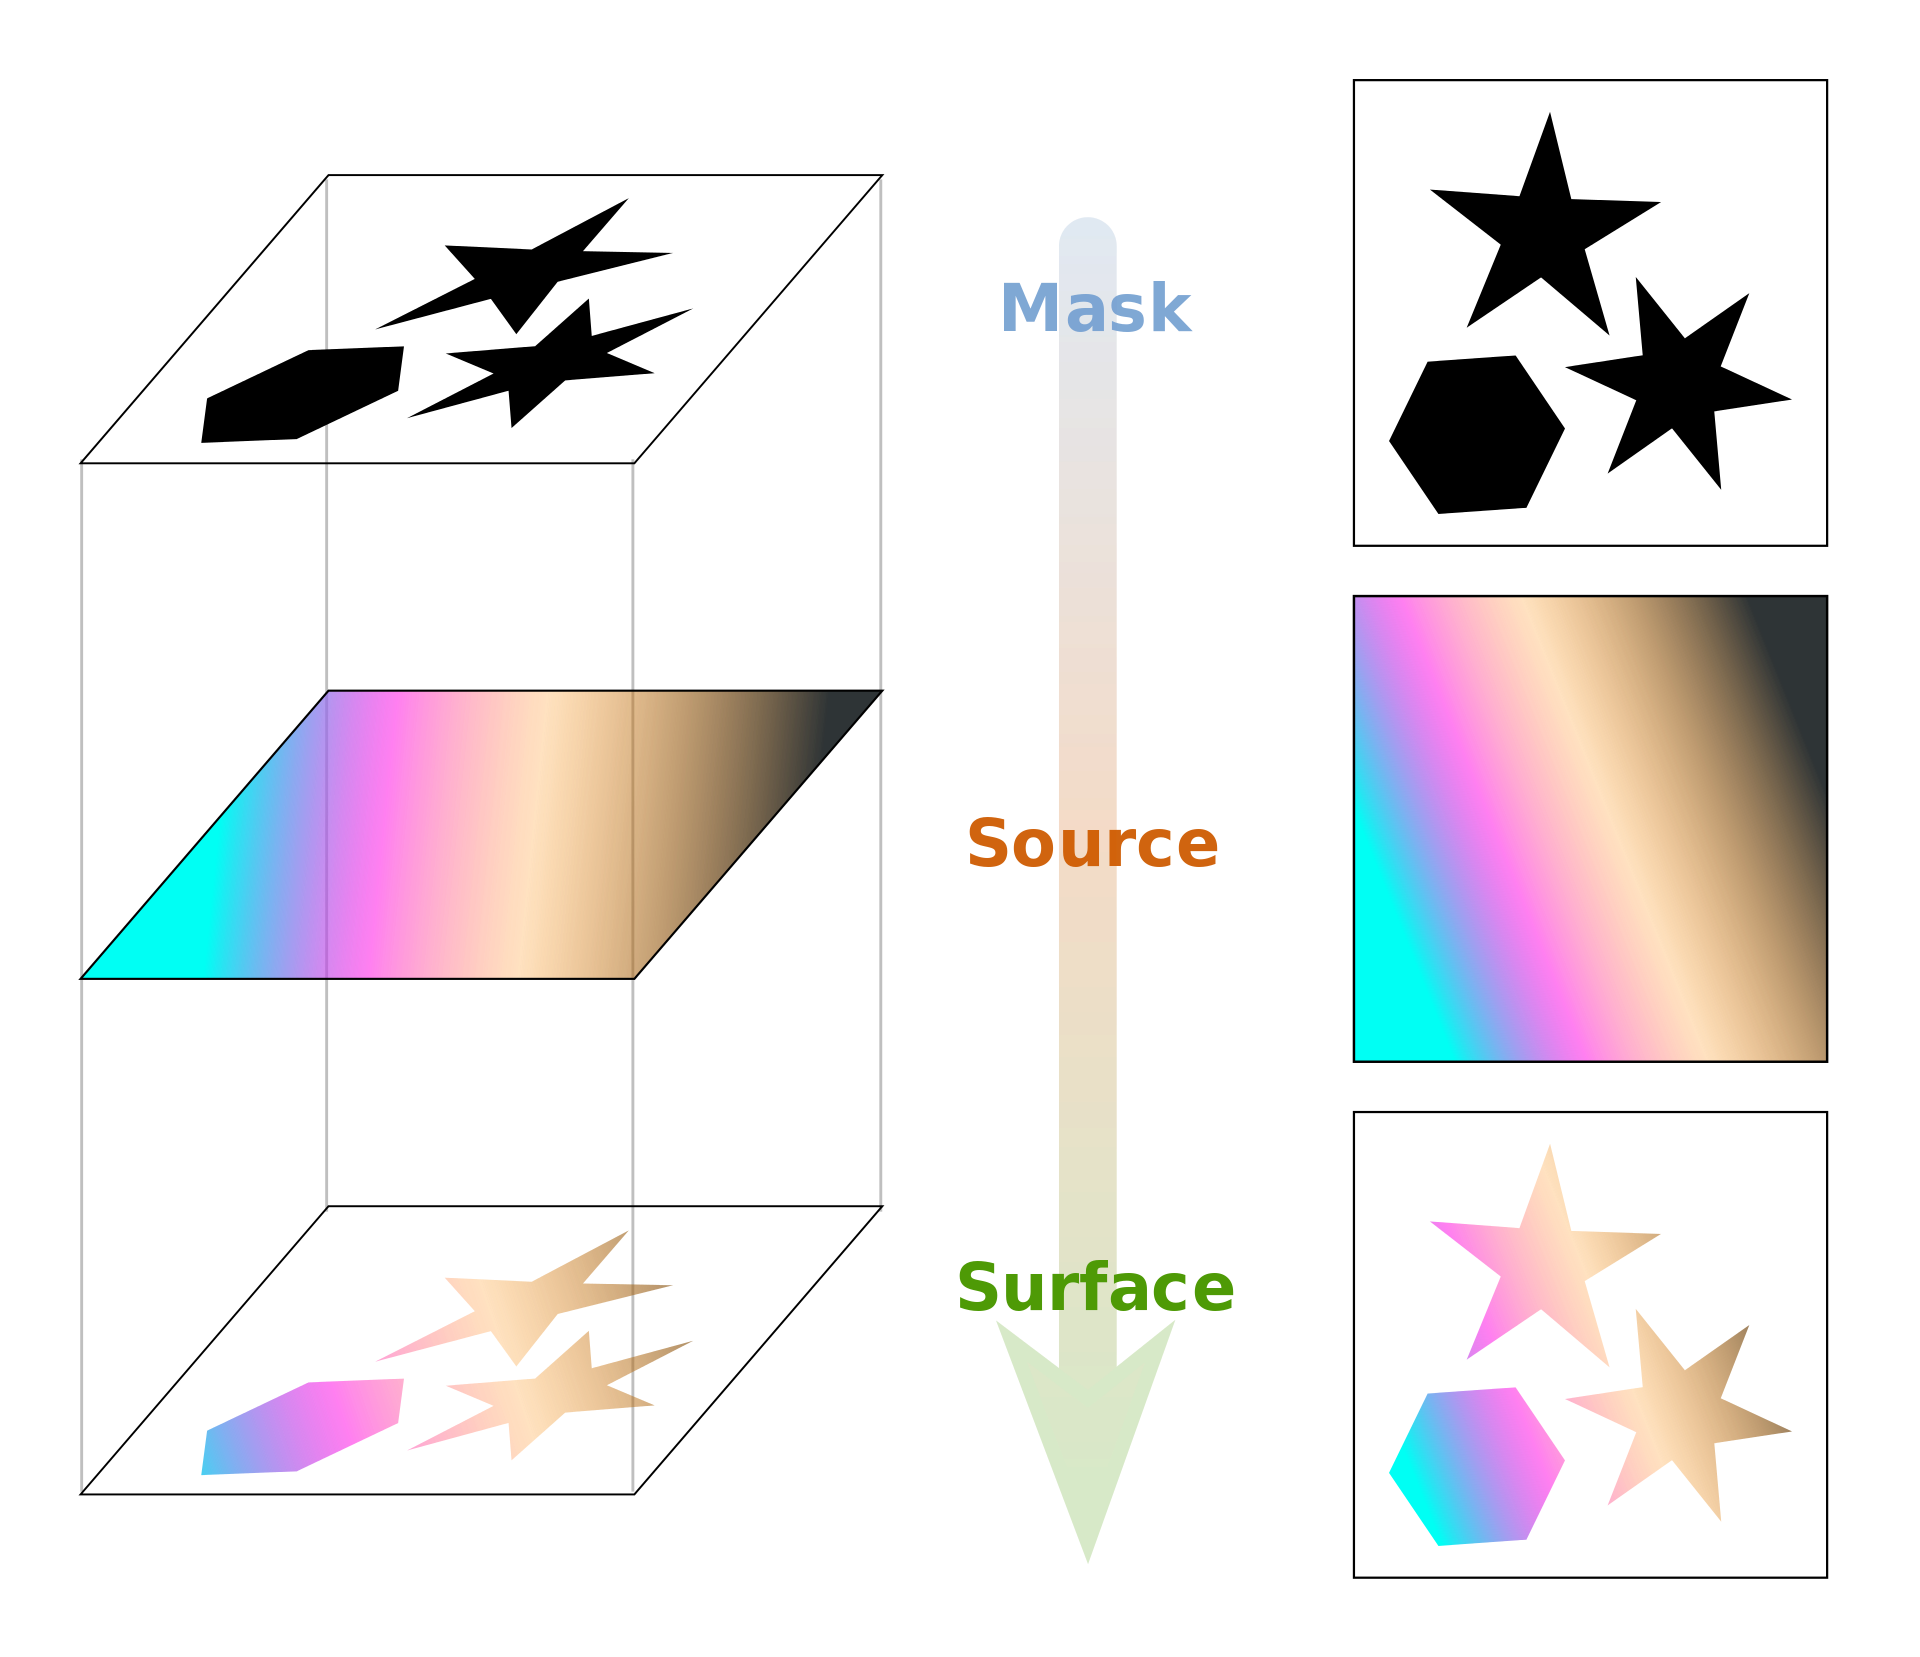
\includegraphics[width=0.6\textwidth]{cairo_model.png}
    \caption{Cairo drawing model (taken from Wikipedia)}
    \label{fig:CairoModel}
\end{figure}

\newpage

\subsection{Implementing the DPD method}

\newpage
\section{Optimizing the Simulation}
\subsection{Computational cost}
\subsection{Cell list}

\newpage
\section{Conclusion}

\newpage
\section{Appendix}

%%%%%
\newpage
\bibliographystyle{unsrt}
\bibliography{references}

\end{document}